\begin{savequote}[45mm]
\ascii{Any fool can write code that a computer can understand. Good programmers write code that humans can understand.}
\qauthor{\ascii{- Martin Flower}}
\end{savequote}

\chapter{MonitoredSession} 
\label{ch:monitored-session}

\begin{content}

训练一个简单的模型,可以通过运行\code{train\_op}数次直至模型收敛,最终将训练参数实施\ascii{Checkpoint},持久化训练模型。对于小规模的学习模型,这个过程至多需要花费数小时的时间。

但是,对于大规模的学习模型,需要花费数天时间;而且可能需要使用多份复本\ascii{(replica)},此时需要更加健壮的训练过程支持模型的训练。因此,需要解决三个基本问题:

\begin{enum}
  \eitem{当训练过程异常关闭,或程序崩溃,能够合理地处理异常;}
  \eitem{当异常关闭,或程序崩溃之后,能够恢复训练过程;} 
  \eitem{能够通过\ascii{TensorBoard}监控整个训练过程。}   
\end{enum}

当训练被异常关闭或程序崩溃之后,为了能够恢复训练过程,必须周期性实施\ascii{Checkpoint}。当训练过程重启后,可以通过寻找最近一次的\ascii{Checkpoint}文件,恢复训练过程。

为了能够使用\ascii{TensorBoard}监控训练过程,可以通过周期性运行一些\ascii{Summary}的\ascii{OP},并将结果追加到事件文件中。\ascii{TensorBoard}能够监控和解析事件文件的数据,可视化整个训练过程,包括展示计算图的结构。

\end{content}

\section{引入MonitoredSession}

\begin{content}

\code{tf.train.MonitoredSession},它可以定制化\code{Hook},用于监听整个\code{Session}的生命周期;内置\code{Coordinator}对象,用于协调所有运行中的线程同时停止,并监听,上报和处理异常;当发生\code{AbortedError}或\code{UnavailableError}异常时,可以重启\code{Session}。

\subsection{使用方法}

一般地,首先使用\code{ChiefSessionCreator}创建\code{Session}实例,并且注册三个最基本的\code{tf.train.SessionRunHook}:

\begin{enum}
  \eitem{\code{CheckpointSaverHook}:周期性地\ascii{Checkpoint};}
  \eitem{\code{SummarySaverHook}:周期性地运行\ascii{Summary};} 
  \eitem{\code{StepCounterHook}:周期性地统计每秒运行的\ascii{Step}数目。}   
\end{enum}

为了能够安全处理异常,并且能够关闭\code{MonitoredSession},常常使用\code{with}的上下文管理器。

\begin{leftbar}
\begin{python}
session_creator = tf.train.ChiefSessionCreator(
  checkpoint_dir=checkpoint_dir,
  master=master,
  config=config)

hooks = [
  tf.train.CheckpointSaverHook(
    checkpoint_dir=checkpoint_dir,
    save_secs=save_checkpoint_secs),
  tf.train.SummarySaverHook(
    save_secs=save_summaries_secs,
    output_dir=checkpoint_dir),
  tf.train.StepCounterHook(
    output_dir=checkpoint_dir, 
    every_n_steps=log_step_count_steps)
]

with tf.train.MonitoredSession(
  session_creator=session_creator,
  hooks=hooks) as sess:
  if not sess.should_stop():
    sess.run(train_op)
\end{python}
\end{leftbar}

\subsection{使用工厂}

使用\code{MonitoredTrainingSession}的工厂方法,可以简化\code{MonitoredSession}的创建过程。

\begin{figure}[!htbp]
\centering
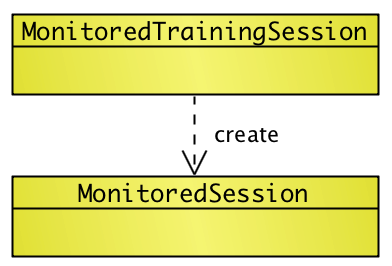
\includegraphics[width=0.4\textwidth]{figures/py-train-monitored-training-session.png}
\caption{MonitoredTrainingSession:工厂方法}
 \label{fig:py-train-monitored-training-session}
\end{figure}

\begin{leftbar}
\begin{python}
with MonitoredTrainingSession(
  master=master,
  is_chief=is_chief,
  checkpoint_dir=checkpoint_dir
  config=config) as sess:
  if not sess.should_stop():
    sess.run(train_op)
\end{python}
\end{leftbar}

\subsection{装饰器}

为了得到复合功能的\code{MonitoredSession},可以将完成子功能的\code{WrappedSession}进行组合拼装。

\begin{enum}
  \eitem{\code{RecoverableSession}:当发生\code{AbortedError}或\code{UnavailableError}异常时,可以恢复和重建\code{Session};}
  \eitem{\code{CoordinatedSession}:内置\code{Coordinator}对象,用于协调所有运行中的线程同时停止,并监听,上报和处理异常;} 
  \eitem{\code{HookedSession}:可以定制化\code{Hook},用于监听整个\code{Session}的生命周期。}   
\end{enum}

\begin{figure}[!htbp]
\centering
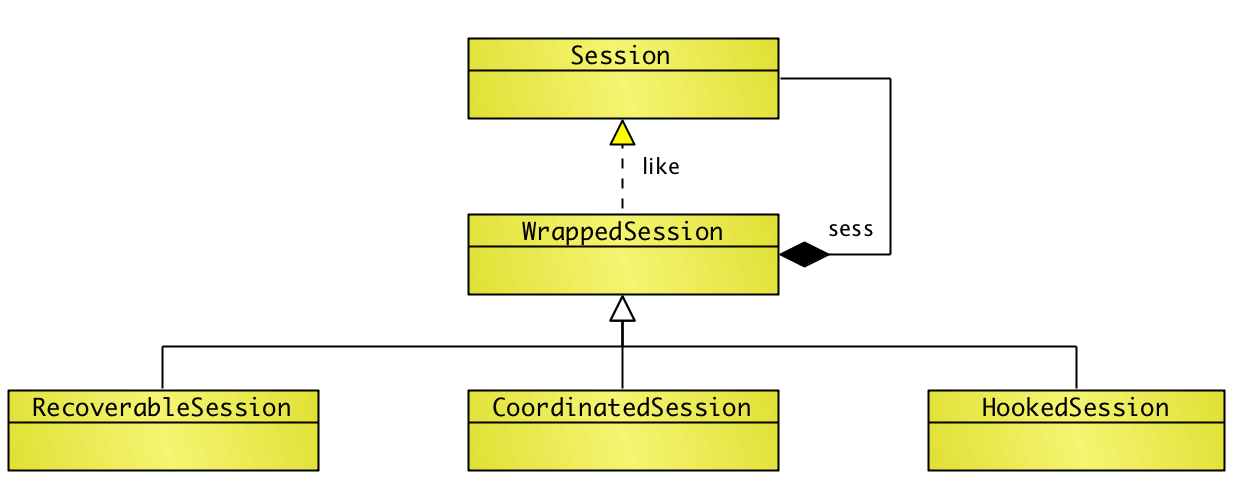
\includegraphics[width=0.9\textwidth]{figures/py-train-monitored-session-decorator.png}
\caption{MonitoredSession:装饰器}
 \label{fig:py-train-monitored-session-decorator}
\end{figure}

最终,可以组合三者的特性,构建得到\code{MonitoredSession}(伪代码实现,详情请查阅\code{MonitoredSession}的具体实现)。

\begin{leftbar}
\begin{python}
MonitoredSession(
  RecoverableSession(
    CoordinatedSession(
      HookedSession(
        tf.Session(target, config)))))
\end{python}
\end{leftbar}

\end{content}

\section{生命周期}

\begin{content}

\code{MonitoredSession}具有\code{Session}的生命周期特征(但并非\ascii{IS-A}关系,而是\ascii{Like-A}关系,这是一种典型的按照鸭子编程的风格)。

在生命周期过程中,插入了\code{SessionRunHook}的回调钩子,用于监听\code{MonitoredSession}的生命周期过程。

\subsection{初始化}

在初始化阶段,\code{MonitoredSession}主要完成如下过程:

\begin{enum}
  \eitem{运行所有回调钩子的\code{begin}方法;}
  \eitem{通过调用\code{scaffold.finalize()}冻结计算图;} 
  \eitem{创建会话:使用\code{SessionCreator}多态创建\code{Session}}   
  \eitem{运行所有回调钩子的\code{after\_create\_session}方法}
\end{enum}

其中,使用\code{SessionCreator}多态创建\ascii{Session}的过程,存在两种类型。

\begin{enum}
  \eitem{\code{ChiefSessionCreator}:调用\code{SessionManager.prepare\_session},通过从最近的\ascii{Checkpoing}恢复模型,或运行\code{init\_op},完成模型的初始化;然后,启动所有\code{QueueRunner}实例;}
  \eitem{\code{WorkerSessionCreator}:调用\code{SessionManager.wait\_for\_session},等待\code{Chief}完成模型的初始化。} 
\end{enum}

\begin{figure}[!htbp]
\centering
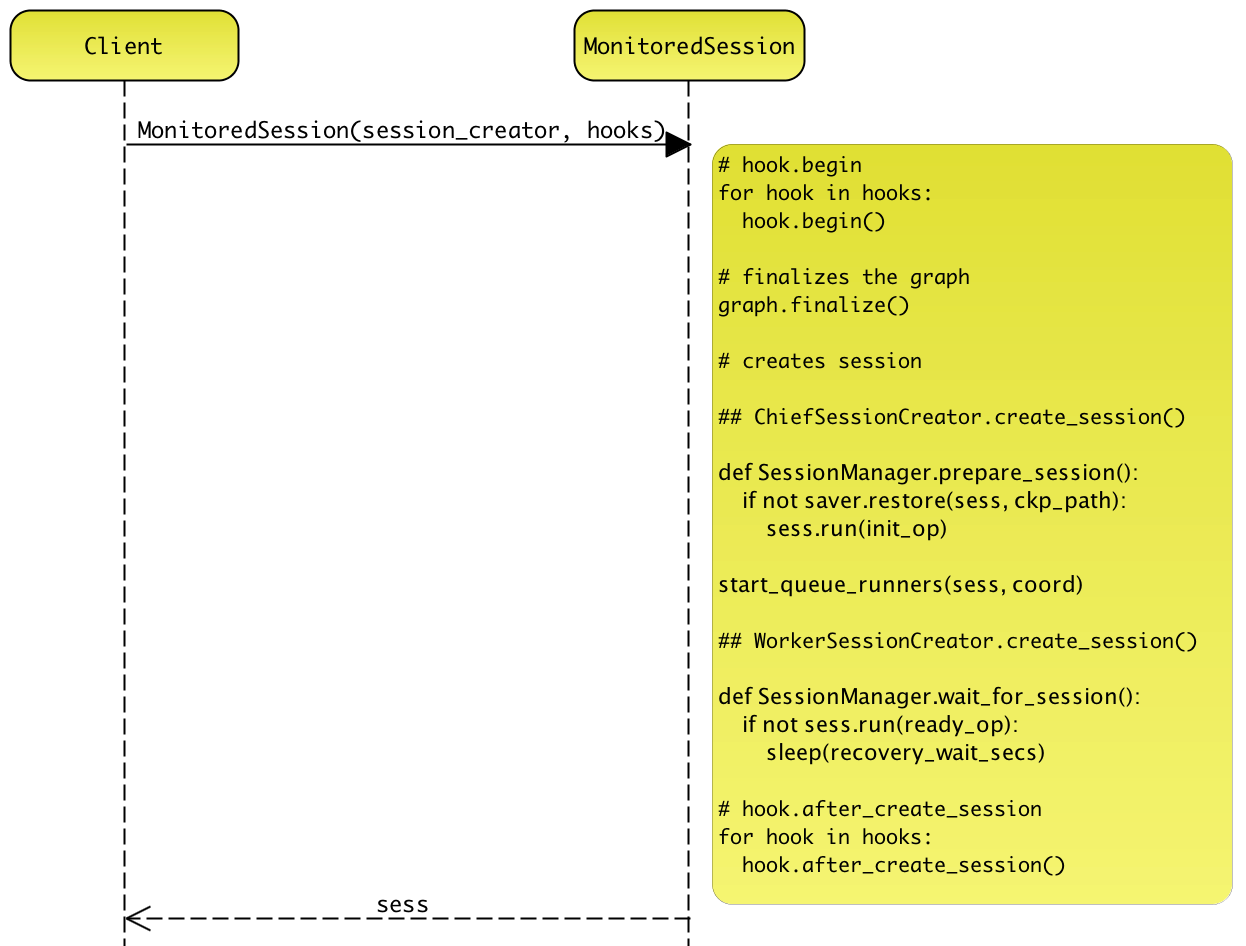
\includegraphics[width=0.9\textwidth]{figures/py-train-monitored-session-initialization.png}
\caption{MonitoredSession:初始化}
 \label{fig:py-train-monitored-session-initialization}
\end{figure}

\subsection{执行}

在执行阶段,在运行\code{Session.run}前后分别回调钩子的\code{before\_run}和\code{after\_run}方法。如果在运行过程发生了\code{AbortedError}或\code{UnavailableError}异常,则重启会话服务。

\begin{figure}[!htbp]
\centering
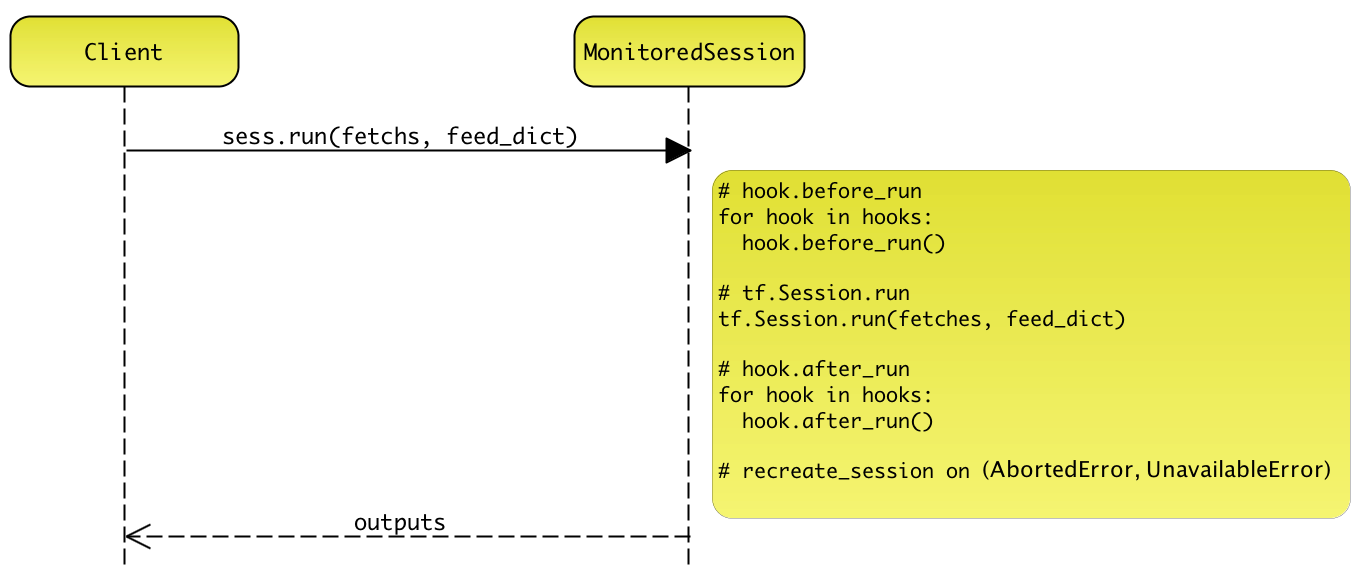
\includegraphics[width=0.9\textwidth]{figures/py-train-monitored-session-execution.png}
\caption{MonitoredSession:执行}
 \label{fig:py-train-monitored-session-execution}
\end{figure}

\subsection{关闭}

当训练过程结束后,通过调用\code{close}方法,关闭\code{MonitoredSession},释放系统的计算资源。

此时,将回调钩子的\code{end}方法,并且会通过调用\code{Coordinator.request\_stop}方法,停止所有\code{QueueRunner}实例。最终,听过调用\code{tf.Session.close}方法,释放系统的资源。

另外,如果发生\code{OutOfRangeError}异常,\code{MonitoredSession}认为训练过程正常终止,并忽略该异常。

\begin{figure}[!htbp]
\centering
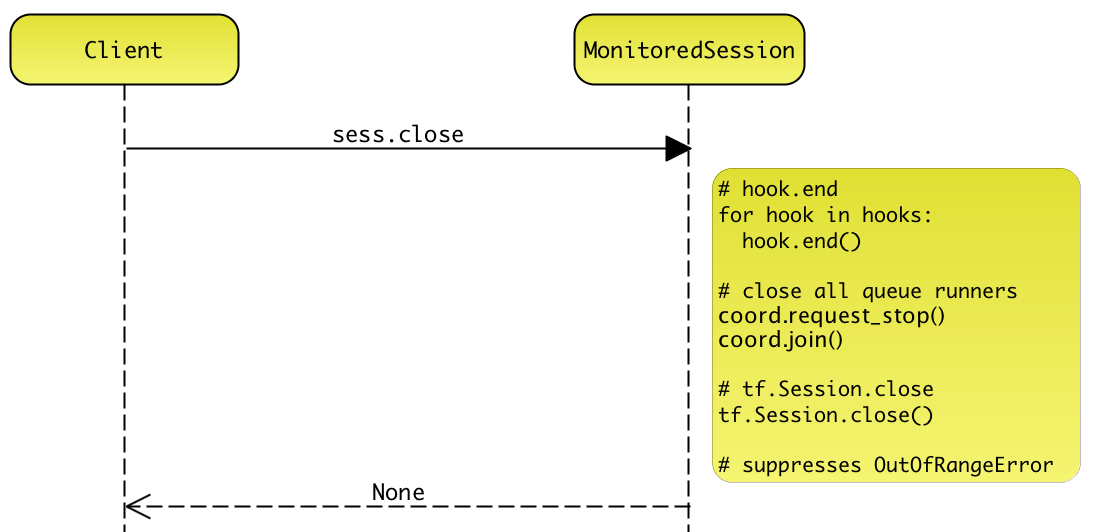
\includegraphics[width=0.9\textwidth]{figures/py-train-monitored-session-close.png}
\caption{MonitoredSession:关闭}
 \label{fig:py-train-monitored-session-close}
\end{figure}

\end{content}

\section{模型初始化}

\begin{content}

\code{MonitoredSession}在初始化时,使用\code{SessionCreator}完成会话的创建和模型的初始化。

一般地,在分布式环境下,存在两中类型的\ascii{Worker}:

\begin{enum}
  \eitem{\ascii{Chief}: 负责模型的初始化;}
  \eitem{\ascii{Non-Chief}: 等待\ascii{Chief}完成模型的初始化。} 
\end{enum}

两者之间,通过一个简单的协调协议共同完成模型的初始化。

\subsection{协调协议}

对于\ascii{Chief},它会尝试从\ascii{Checkpoint}文件中恢复模型;如果没有成功,则会通过执行\code{init\_op}全新地初始化模型;其初始化算法,可以形式化描述为:

\begin{leftbar}
\begin{python}
def prepare_session(master, init_op, saver, ckp_dir):
  if is_chief():
    sess = tf.Session(master)
    sess.run(init_op) if not saver.restore(sess, ckp_dir)
\end{python}
\end{leftbar}

对于\ascii{Non-Chief},它会周期性地通过运行\ascii{ready\_op},查看\ascii{Chief}是否已经完成模型的初始化。

\begin{leftbar}
\begin{python}
def wait_for_session(master, ready_op, recovery_wait_secs):
  while True:
    sess = tf.Session(master)
    if sess.run(ready_op):
      return sess
    else:
      sess.close()
      time.sleep(recovery_wait_secs)   
\end{python}
\end{leftbar}

\subsection{SessionManager}

事实上,上述算法主要由\code{SessionManager}实现,它主要负责从\ascii{Checkpoint}文件中完成模型的恢复,或直接通过运行\code{init\_op}完成模型的初始化,最终创建可工作的\code{Session}实例。

\begin{enum}
  \eitem{对于\ascii{Chief},通过调用\code{prepare\_session}方法,完成模型的初始化;}
  \eitem{对于\ascii{Non-Chief},通过调用\code{wait\_for\_session}方法,等待\ascii{Chief}完成模型的初始化。} 
\end{enum}

详情可以参考\code{SessionManager}的具体实现。

\subsection{引入工厂}

使用工厂方法,分别使用\code{ChiefSessionCreator}和\code{WorkerSessionCreator}分别完成上述算法。

\begin{figure}[!htbp]
\centering
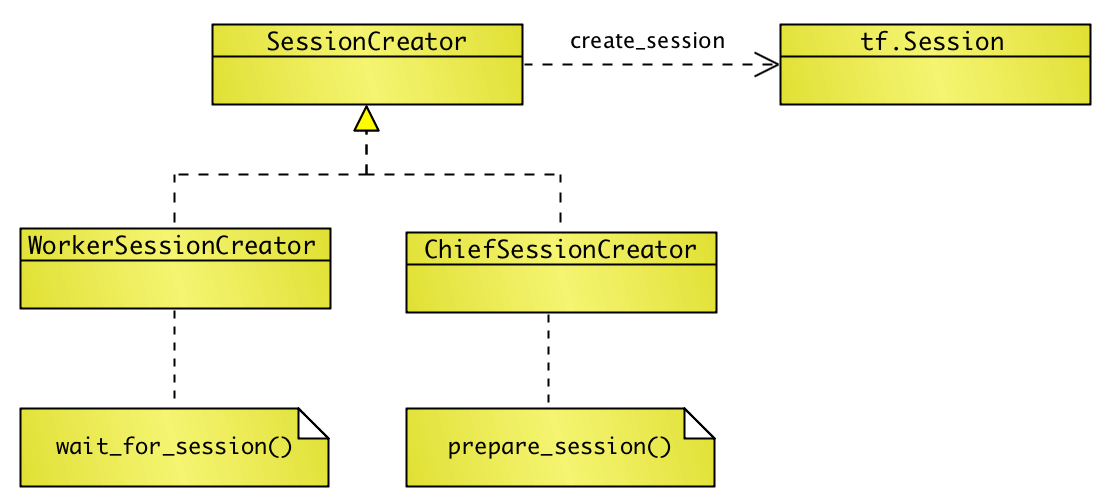
\includegraphics[width=0.9\textwidth]{figures/py-train-session-creator.png}
\caption{SessionManager}
 \label{fig:py-train-session-creator}
\end{figure}

\subsection{Scaffold}

当要构建一个模型训练,需要\code{init\_op}初始化变量;需要\code{Saver}周期性实施\ascii{Checkpoint};需要\code{ready\_op}查看一个模型是否已经初始化完毕;需要\code{summary\_op}搜集所有\ascii{Summary},用于训练过程的可视化。

一般地,在计算图中通过\code{GraphKey}标识了这些特殊的OP或对象,以便可以从计算图中检索出这些特殊的\ascii{OP}或对象。

在训练模型的特殊领域中,提供了一个基础工具库:\code{Scaffold},用于创建这些\ascii{OP}或对象的默认值,并添加到计算图的集合中,并且\code{Scaffold}提供了查询接口可以方便地获取到这些\ascii{OP}或对象。

可以通过调用\code{Scaffold.finalize}方法,如果对应的\ascii{OP}或对象为\code{None},则默认创建该类型的实例。最终冻结计算图,之后禁止再往图中增加节点。

\begin{leftbar}
\begin{python}
class Scaffold(object):
  def finalize(self):
    """Creates operations if needed and finalizes the graph."""
    
    # create init\_op
    if self._init_op is None:
      def default_init_op():
        return control_flow_ops.group(
            variables.global_variables_initializer(),
            resources.initialize_resources(
              resources.shared_resources()))
      self._init_op = Scaffold.get_or_default(
          'init_op',
          ops.GraphKeys.INIT_OP,
          default_init_op)

    # create ready\_op
    if self._ready_op is None:
      def default_ready_op():
        return array_ops.concat([
            variables.report_uninitialized_variables(),
            resources.report_uninitialized_resources()
        ], 0)
      self._ready_op = Scaffold.get_or_default(
          'ready_op', 
          ops.GraphKeys.READY_OP,
          default_ready_op)
    
    # create ready\_for\_local\_init\_op
    if self._ready_for_local_init_op is None:
      def default_ready_for_local_init_op():
        return variables.report_uninitialized_variables(
            variables.global_variables())
      self._ready_for_local_init_op = Scaffold.get_or_default(
          'ready_for_local_init_op',
          ops.GraphKeys.READY_FOR_LOCAL_INIT_OP,
          default_ready_for_local_init_op)
    
    # create local\_init\_op
    if self._local_init_op is None:
      def _default_local_init_op():
        return control_flow_ops.group(
            variables.local_variables_initializer(),
            lookup_ops.tables_initializer())
      self._local_init_op = Scaffold.get_or_default(
          'local_init_op',
          ops.GraphKeys.LOCAL_INIT_OP,
          _default_local_init_op)
    
    # create summary\_op
    if self._summary_op is None:
      self._summary_op = Scaffold.get_or_default(
          'summary_op',
          ops.GraphKeys.SUMMARY_OP,
          summary.merge_all)
    
    # create Saver
    if self._saver is None:
      self._saver = training_saver._get_saver_or_default()
    self._saver.build()

    ops.get_default_graph().finalize()
    return self
\end{python}
\end{leftbar}

从\code{finalize}的实现可以看出,以下\ascii{OP}完成的功能为:

\begin{enum}
  \eitem{\code{init\_op}: 完成所有全局变量和全局资源的初始化;}
  \eitem{\code{local\_init\_op}: 完成所有本地变量和表格的初始化;} 
  \eitem{\code{ready\_op}: 查看所有的全局变量和全局资源是否已经初始化了;否则报告未初始化的全局变量和全局资源的列表;}   
  \eitem{\code{ready\_for\_local\_init\_op}: 查看所有的本地变量和表格是否已经初始化了;否则报告未初始化的本地变量和表格的列表;}   
  \eitem{\code{summary\_op}: 汇总所有\ascii{Summary}的输出;}       
\end{enum}

其中,本地变量不能持久化到\ascii{Checkpoint}文件中;当然,也就不能从\ascii{Checkpoint}文件中恢复本地变量的值。

\subsection{初始化算法}

通过观测上面的\ascii{OP}的定义,理解\code{prepare\_session}模型初始化的完整语义便不是那么困难了。

\begin{leftbar}
\begin{python}
class SessionManager(object):
  def prepare_session(self,
                      master,
                      saver=None
                      checkpoint_filename=None
                      init_op=None,
                      init_feed_dict=None,
                      init_fn=None):
    """Creates a Session. Makes sure the model is ready."""

    def _restore_checkpoint():
      sess = session.Session(master)
      if not saver or not checkpoint_filename):
        return sess, False
      else:
        saver.restore(sess, checkpoint_filename)
        return sess, True

    def _try_run_init_op(sess):
      if init_op is not None:
        sess.run(init_op, feed_dict=init_feed_dict)
      if init_fn:
        init_fn(sess)
    
    sess, is_succ = self._restore_checkpoint()
    if not is_succ:
      _try_run_init_op(sess)
    self._try_run_local_init_op(sess)
    self._model_ready(sess)
    return sess
\end{python}
\end{leftbar}

其初始化算法非常简单。首先,尝试从\ascii{Checkpoint}文件中恢复(此处为了简化问题,省略了部分实现);如果失败,则调用\code{init\_op}和\code{init\_fn}完成全局变量和资源的初始化;然后,才能实施本地变量和表格的初始化;最后,验证所有全局变量和资源是否已经初始化了。

\begin{figure}[!htbp]
\centering
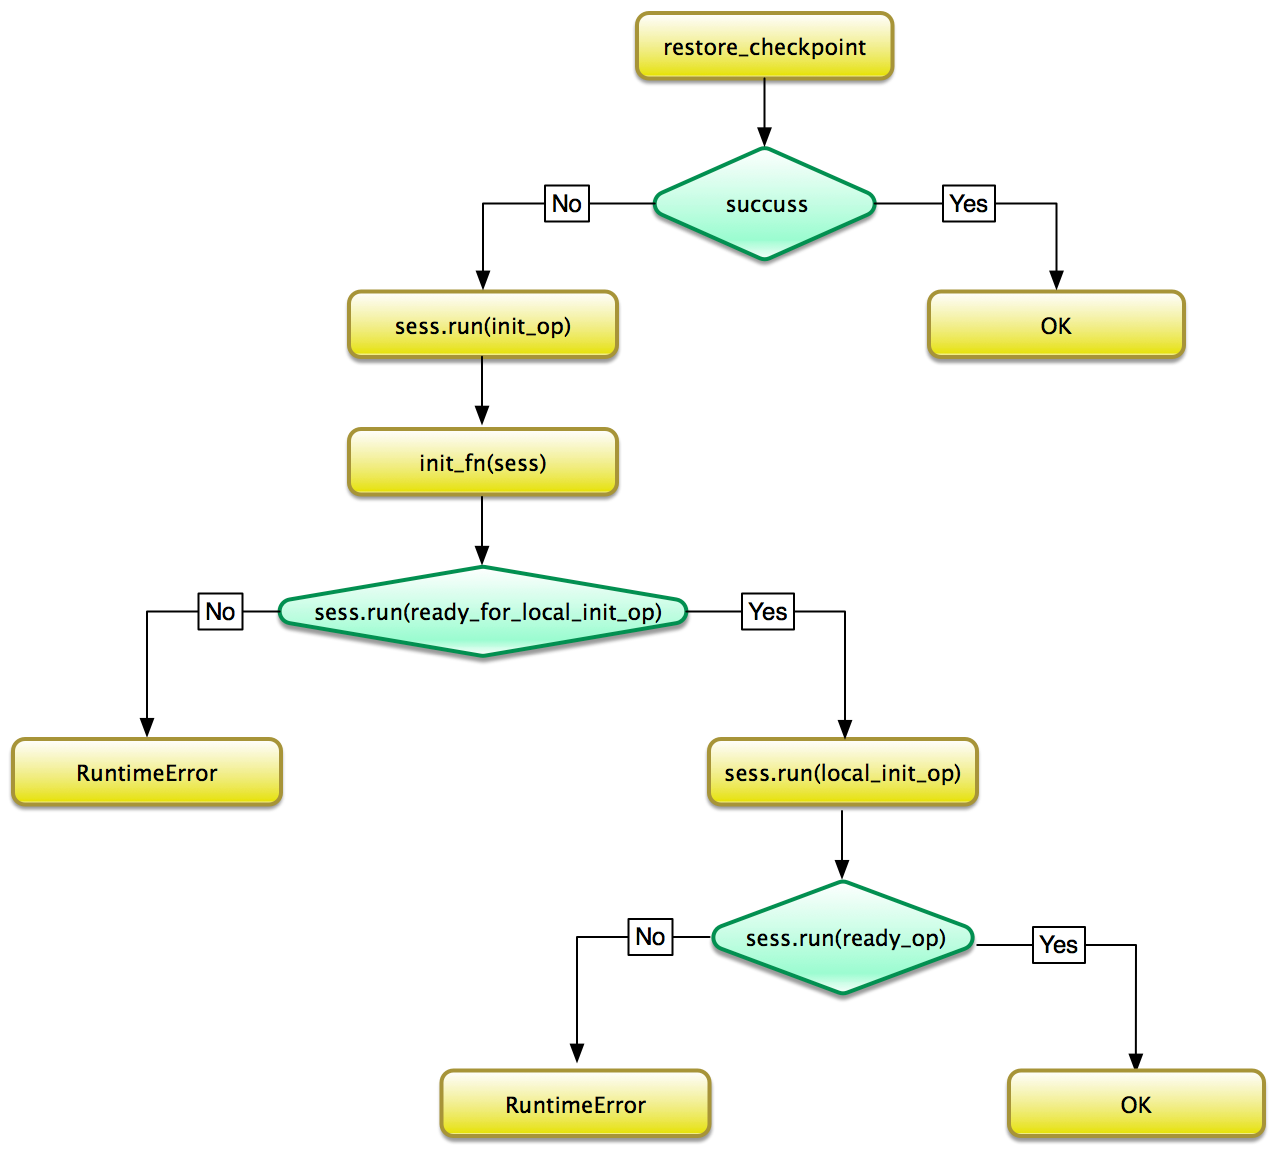
\includegraphics[width=0.9\textwidth]{figures/py-train-session-initialization-algo.png}
\caption{模型初始化算法}
 \label{fig:py-train-session-initialization-algo}
\end{figure}

\subsection{本地变量初始化}

对于非空的\code{local\_init\_op},必须等所有全局变量已经初始化完毕后才能进行初始化(通过调用\code{\_ready\_for\_local\_init\_op});否则,报告未初始化的全局变量列表到\code{msg}字段中。

也就是说,本地变量初始化在全局变量初始化之后,且本地变量不会持久化到\ascii{Checkpoint}文件中。

\begin{leftbar}
\begin{python}
class SessionManager(object):
  def _ready_for_local_init(self, sess):
    """Checks if the model is ready to run local_init_op.
    """
    return _ready(self._ready_for_local_init_op, sess,
                  "Model not ready for local init")

  def _try_run_local_init_op(self, sess):
    """Tries to run _local_init_op, if not None, 
       and is ready for local init.
    """
    if not self._local_init_op:
      return True, None:
    
    is_ready, msg = self._ready_for_local_init(sess)
    if is_ready:
      sess.run(self._local_init_op)
      return True, None
    else:
      return False, msg
\end{python}
\end{leftbar}

\subsection{验证模型}

最后,通过执行\code{\_ready\_op},查看所有全局变量和全局资源是否都已经初始化了;否则,报告未初始化的变量列表到\code{msg}字段中。

\begin{leftbar}
\begin{python}
class SessionManager(object):
  def _model_ready(self, sess):
    """Checks if the model is ready or not.
    """
    return _ready(self._ready_op, sess, "Model not ready")
\end{python}
\end{leftbar}

其中,\code{\_ready}使用函数,用于运行相应的\code{ready\_op},查看相应的变量或资源是否完成初始化。

\begin{leftbar}
\begin{python}
def _ready(op, sess, msg):
  """Checks if the model is ready or not, as determined by op.
  """
  if op is None:
    return True, None

  ready_value = sess.run(op)
  if (ready_value.size == 0):
    return True, None
  else:
    uninitialized_vars = ", ".join(
        [i.decode("utf-8") for i in ready_value])
    return False, "initialized vars: " + uninitialized_vars
\end{python}
\end{leftbar}

\end{content}

\section{异常安全}

\begin{content}

一般地,常常使用\code{with}的上下文管理器,实现\code{MonitoredSession}的异常安全和资源安全释放。

\subsection{上下文管理器}

当退出\code{with}语句后,将停止运行所有\code{QueueRunner}实例,并实现\code{tf.Session}的安全关闭。

\begin{leftbar}
\begin{python}
class _MonitoredSession(object):
  def __exit__(self, exception_type, exception_value, traceback):
    if exception_type in [errors.OutOfRangeError, StopIteration]:
      exception_type = None
    self._close_internal(exception_type)
    return exception_type is None
  
  def _close_internal(self, exception_type=None):
    try:
      if not exception_type:
        for h in self._hooks:
          h.end(self.tf_sess)
    finally:
      try:
        self._sess.close()
      finally:
        self._sess = None
        self.tf_sess = None
        self.coord = None  
\end{python}
\end{leftbar}

特殊地,当发生\code{OutOfRangeError}或\code{StopIteration},则认为正常终止,忽视该异常。如果抛出了其它类型的异常,则不会调用\code{end}的回调钩子。

\subsection{停止QueueRunner}

另外,当执行\code{self.\_sess.close()},最终将调用\code{\_CoordinatedSession}的\code{close}方法。通过调用\code{coord.request\_stop}通知所有\code{QueueRunner}实例停止运行,并且通过调用\code{coord.join}方法等待所有\code{QueueRunner}实例运行完毕。

\begin{leftbar}
\begin{python}
class _CoordinatedSession(_WrappedSession):
  def close(self):
    self._coord.request_stop()
    try:
      self._coord.join()
    finally:
      try:
        _WrappedSession.close(self)
      except Exception:
        pass
\end{python}
\end{leftbar}

\end{content}

\section{回调钩子}

\begin{content}

可以通过定制\code{SessionRunHook},实现对\code{MonitorSession}生命周期过程的监听和管理。

\begin{leftbar}
\begin{python}
class SessionRunHook(object):
  def begin(self):
    pass

  def after_create_session(self, session, coord):
    pass

  def before_run(self, run_context):
    return None

  def after_run(self, run_context, run_values):
    pass

  def end(self, session):
    pass
\end{python}
\end{leftbar}

其中,最常见的\code{Hook}包括:

\begin{enum}
  \eitem{\code{CheckpointSaverHook}:周期性地\ascii{Checkpoint};}
  \eitem{\code{SummarySaverHook}:周期性地运行\ascii{Summary};} 
  \eitem{\code{StepCounterHook}:周期性地统计每秒运行的\ascii{Step}数目。}   
\end{enum}

\begin{figure}[!htbp]
\centering
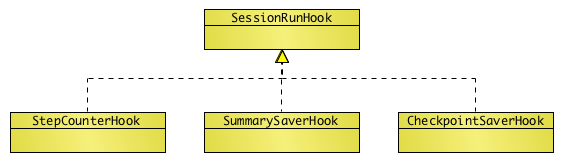
\includegraphics[width=0.9\textwidth]{figures/py-train-session-run-hook.png}
\caption{SessionRunHook}
 \label{fig:py-train-session-run-hook}
\end{figure}

\end{content}






